\chapter[Integrated array tomography]{Integrated array tomography for 3D correlative light and electron microscopy}
\label{chap:3}

% Abstract
\begin{abstract}
    Volume electron microscopy (EM) of biological systems has grown exponentially in recent years due to innovative large-scale imaging approaches. As a standalone imaging method, however, large-scale EM typically has two major limitations: slow rates of acquisition and the difficulty to provide targeted biological information. We developed a 3D image acquisition and reconstruction pipeline that overcomes both of these limitations by using a widefield fluorescence microscope integrated inside of a scanning electron microscope. The workflow consists of acquiring large field of view fluorescence microscopy (FM) images, which guide to regions of interest for successive EM (integrated correlative light and electron microscopy). High precision EM-FM overlay is achieved using cathodoluminescent markers. We conduct a proof-of-concept of our integrated workflow on immunolabelled serial sections of tissues. Acquisitions are limited to regions containing biological targets, expediting total acquisition times and reducing the burden of excess data by tens or hundreds of GBs.
\end{abstract}

% Published as footnote
\blfootnote{This chapter has been published as: \fullcite{lane2022integrated}.}
\clearpage


% Sections
\section{Introduction}
\label{sec:4.1_intro}


% Motivate from EM perspective
% bio-insight from EM is hard
% CLEM has been developed to assist

Electron microscopy (EM) has transformed the way in which biologists understand intra- and inter-cellular systems. Due to the lack of inherent biological specificity, however, interpretation of EM datasets typically requires tedious expert analysis and annotation. For this reason, fluorescence microscopy (FM) is often used in conjunction with EM, complementing structural data with targeted biological labels. Fluorescent labelling, however, comes with several drawbacks. Sample preparation protocols are often laborious, time-consuming, and potentially damaging to the sample. Protocols must also be adapted to limit concentrations of heavy metal staining if intermediate processing of the sample is to be avoided \cite{kuipers2015scanning,lane2021optimization}. Fluorescent labelling is also susceptible to bleedthrough when multiple fluorophores are expressed in a single sample as well as varying specificity---Hoechst dyes, for instance, bind to both DNA and RNA. Furthermore, registering the separate imaging modalities across large spatial extents remains a technically challenging and primarily manual task \cite{russell20173d} [other references]. Correlative fluorescence and electron microscopy experiments are therefore typically limited in scope to the micron or tens of microns scale, and thus so are the regions for which biological labels can be provided \cite{russell20173d} [other references].

As recognition of organelles and other subcellular structures remains a pivotal obstacle in biological EM, we questioned whether large-scale EM datasets could be supplemented with biological labels through alternate means. To address this question, we sought to leverage recent advances in deep learning. Deep convolutional neural networks (CNN) in particular have been shown to be capable of inferring complex, non-linear relationships from image data \cite{he2016deep,januszewski2018high}. Prior work involving deep CNNs in the context of electron microscopy data has primarily been limited to applications in segmentation, denoising, and compressed sensing \cite{ede2021deep}. Semantic segmentation, the classification of pixels into discrete categories, does ultimately serve the purpose of adding biological labels to EM data. However, modern deep learning approaches require hours of tedious expert segmentation \cite{huang2014identifying,heinrich2018synaptic,liu2020automatic,spiers2021deep}. In order for \textcite{heinrich2020automatic} to amass sufficient training data for organelle segmentation, it required one person two weeks of manual segmentation per \SI{1}{\micro\meter^3} volume of image data; 28 blocks of this size were manually annotated in total to enable whole cell organelle segmentation.

Although relatively little attention has been paid to alternative applications in deep learning for EM data, recent work has focused on generating biological labels from other imaging modalities. \textcite{christiansen2018silico} designed a deep neural network to predict fluorescence labels from transmitted light images. \textcite{ounkomol2018label} extended the technique to generate 3D fluorescence from stacks of transmitted light microscopy data and further demonstrated the possibility of predicting immunofluorescence from EM images in order to facilitate automatic registration of fluorescence data with EM. To address the challenge of adding biological specificity to large-scale EM datasets, we thus explored the potential for a CNN to make label-free fluorescence predictions from electron microscopy image data.

In this work we present a deep CNN developed for generating fluorescence predictions on large-scale EM data of tissue and cellular samples. We demonstrate the performance of our model on thin sections of rat pancreas tissue, which have been immunolabelled with Alexa Fluor 594 and given a Hoechst counterstain, as well as Hoechst-stained sections of resin-embedded HeLa cells. Network predictions are quantitatively evaluated against corresponding true fluorescence images based on the Pearson correlation coefficient (PCC, or $\rho$) as well as by assessing human recognition of fluorescence predictions on cell nuclei. We additionally assess the network's robustness by measuring its predictive power on EM datasets acquired with varying imaging parameters. Finally, we explore the potential of correlative and predicted fluorescence signals for use as labels in segmentation experiments.






% \subsection{Things we will show}
% \begin{itemize}[noitemsep]
%     \item Can train a CNN to predict fluorescence based on registered CLEM images as training data
%     \begin{itemize}
%         \item Demonstrate on rat pancreas tissue: cell nuclei and insulin granules (micron scale and sub-diffraction limit)
%         \item Demonstrate on zebrafish: cell nuclei
%         \item Demonstrate on mouse heart tissue: phospholamban labelled with TRITC
%         \item Validate with PCC etc.\ and manual counting (for rat pancreas cell nuclei only)
%     \end{itemize}

%     \item CLEMnet is robust
%     \begin{itemize}
%         \item Predictions can be made on different rats
%         \item Predictions can be made on lower signal images (lower dwell) when trained with noise augmentation
%     \end{itemize}

%     \item CLEMnet predictions can be used for (semi/fully)-automated segmentation
%     \begin{itemize}
%         \item CLEMnet data slightly outperforms CLEM data for segmenting cell nuclei
%         \item Caveat that segmentation falls short of manual segmentation
%     \end{itemize}
% \end{itemize}




% Deep convolutional neural networks (CNN) are capable of inferring complex, non-linear relationships between images. Prior work applying deep learning strategies to EM data has often revolved around segmentation tasks. Competitions such as the IEEE International Symposium on Biomedical Imaging (ISBI) challenge for segmentation of neuronal structures in electron microscopic stacks \cite{arganda2015crowdsourcing} have inspired generations of neural network architecture development such as the U-net \cite{ronneberger2015u} and its 3D counterpart \cite{cciccek20163d}. More recently, a CNN has been employed for for whole cell organelle segmentation in a micron-sized volumetric EM dataset \cite{heinrich2020automatic}. Relatively little attention has been paid to alternative applications of deep learning algorithms for volumetric EM data. \textcite{ounkomol2018label} trained a model to facilitate automatic registration of multichannel fluorescence data to EM array tomography data. % Limited to myelin. [More examples].




% As recognition of organelles and other subcellular structures remains a pivotal obstacle in biological EM, [lots and lots of work] has centered around segmentation and classification of these structures. More recently, these efforts have focused on employing deep learning strategies to infer [descriptive adjective] patterns from EM image data rich in structural information \cite{heinrich2020automatic} [25 references therein]. [only expert-level people would otherwise be capable of discerning].
% %
% Competitions such as the IEEE International Symposium on Biomedical Imaging (ISBI) challenge for segmentation of neuronal structures in electron microscopic stacks \cite{arganda2015crowdsourcing} have inspired generations of neural network architecture development such as the U-net \cite{ronneberger2015u} and its 3D counterpart \cite{cciccek20163d}. More recently, a CNN has been employed for whole cell organelle segmentation in a micron-sized volumetric EM dataset \cite{heinrich2020automatic}.


% %
% [No one(?) is making use of multimodal datasets to assist in recognition and segmentation of EM datasets]. 



\section{Material \& methods}
\label{sec:3.2_methods}


% 3.2.1
% -----
\subsection{Tissue and sample preparation}
\label{sec:3M_prep}
Rat pancreas was prepared as follows: fresh pancreas was cut from an \SI{83}{day} old rat into small pieces and fixed in 4\% paraformaldehyde (PFA; Merck) + 0.1\% glutaraldehyde (GA; Polysciences) as described in \textcite{ravelli2013destruction}. A complete zebrafish larva (\SI{120}{hpf}) was fixed in 2\% PFA + 2\% GA. Both samples were post-fixed in 1\% osmium tetroxide and 1.5\% potassium ferricyanide in \SI{0.1}{M} cacodylate buffer, dehydrated through ethanol and embedded in EPON (Serva). \SI{100}{\nano\meter} serial sections were cut and placed onto formvar-covered ITO-coated glass coverslips (Optics Balzers). Immunolabeling was performed as described previously \cite{kuipers2015scanning}. Samples were etched with 1\% periodic acid for \SI{10}{\minute}, followed by a \SI{30}{\minute} blocking step: 1\% bovine serum albumin (BSA; Sanquin, Netherlands) in tris-buffered saline (TBS), pH 7.4. Next, anti-insulin was incubated for \SI{2}{\hour} (guinea pig; 1:50, Invitrogen, PA1-26938, RRID: AB\_794668, for rat pancreas and anti-insulin; 1:100, Abcam, ab210560, for zebrafish pancreas), followed by washing and subsequent incubation for \SI{1}{\hour} with biotinylated secondary antibody (donkey-anti-guinea pig; 1:400, Jackson Immunoresearch, for rat pancreas and goat-anti-rabbit; 1:400, Dako, for zebrafish pancreas) followed by washing steps. Finally, streptavidin conjugated AF594 (1:100, Jackson Immunoresearch, for rat pancreas) and streptavidin conjugated TRITC (1:100, Jackson Immunoresearch, for zebrafish pancreas) were added for \SI{1}{\hour} followed by washing.


% 3.2.2
% -----
\subsection{Digital light microscopy}
\label{sec:3M_keyence}
The sections, after being placed on the ITO-coated glass slide, are imaged at \SI{30}{X} magnification (${\sim}$\SI{7}{\micro\meter\per\pixel}) using a VHX-6000 digital light microscope (Keyence) operating in reflection mode. To capture every section on the \SI{22}{\milli\meter} $\times$ \SI{22}{\milli\meter} ITO-coated glass slide, a 3 $\times$ 3 grid of RGB images is acquired and automatically stitched together.


% 3.2.3
% -----
\subsection{Integrated microscopy}
\label{sec:3M_integrated}
The integrated microscope is a widefield SECOM fluorescence microscope (Delmic B.V.) retrofitted into the vacuum chamber of a Verios 460 SEM (Thermo Fisher Scientific) \cite{liv2013simultaneous, zonnevylle2013integration}. The microscopes share a common optical axis, translation stage, and control software. FM images are obtained with \SI{10}{\second} exposures, recorded by a Zyla 4.2 sCMOS camera (Andor - Oxford Instruments). Excitation wavelengths of \SI{405}{\nano\meter} and \SI{555}{\nano\meter} are used to excite Hoechst and AF594. The SECOM is equipped with a CFI S Plan Fluor ELWD 60XC (\SI{0.70}{NA}) objective (Nikon), which allows for long working distance imaging (\SIrange{1.8}{2.6}{\milli\meter}), to prevent electrical breakdown in vacuum, which must be accounted for due to the presence of high electric fields induced by the stage bias \cite{vos2021retarding}.

SEM imaging is conducted in two rounds: (1) low-magnification (\SI{38}{\nano\meter\per\pixel}) scans accompanying each fluorescent acquisition; (2) high-magnification (\SI{5}{\nano\meter\per\pixel}) acquisitions on ROI identified by fluorescence expression. Both low and high magnification imaging are performed at \SI{2.5}{\kilo\electronvolt} primary beam energy with a \SI{-1}{\kilo\volt} bias potential applied to the sample stage such that the landing energy is \SI{1.5}{\kilo\electronvolt}, which proved optimal for ${\sim}$\SI{100}{\nano\meter} sections. The negative potential bias enhances the backscattered electron (BSE) signal, which is collected by the insertable concentric backscattered detector (Thermo Fisher Scientific) \cite{lane2021optimization}.


% 3.2.4
% -----
\subsection{Alignment and reconstruction software}
Image data from the integrated microscope is uploaded to a local storage server running an instance of render-ws,\footnote{\href{https://github.com/saalfeldlab/render}{https://github.com/saalfeldlab/render}} a collection of open-source web services for rendering transformed image tiles. The tiles and their respective metadata are organized into stacks, configured as MongoDB databases. The alignment routines are arranged in a series of Jupyter notebooks,\footnote{\href{https://github.com/hoogenboom-group/iCAT-workflow}{https://github.com/hoogenboom-group/iCAT-workflow}} which parse the image metadata for the EM-FM overlay as well as make calls to render-ws via a python wrapper (render-python\footnote{\href{https://github.com/AllenInstitute/render-python}{https://github.com/AllenInstitute/render-python}}). EM image stitching and volume alignment are based on the scale-invariant feature transform (SIFT)---an algorithm designed to detect and match local features in corresponding images \cite{lowe1999object}. SIFT features are stored in render-ws databases where they can be processed by BigFeta,\footnote{\href{https://github.com/AllenInstitute/BigFeta}{https://github.com/AllenInstitute/BigFeta}} a linear least squares solver for scalable 2D and 3D image alignment based on point correspondences. CLEM datasets are ultimately exported to CATMAID \cite{saalfeld2009catmaid} for google-maps-like visualization. 3D visualizations are done in Fiji \cite{schindelin2012fiji} using the Volume Viewer plugin.\footnote{\href{https://imagej.net/plugins/volume-viewer}{https://imagej.net/plugins/volume-viewer}}

\section{Results}
\label{sec:3.3_results}


\section{Discussion}
\label{sec:3.4_discussion}

A new workflow for integrated array tomography for the semi-automated acquisition and reconstruction of volume CLEM data is presented. High-resolution EM is limited to select ROI by targeting areas based on fluorescence expression. This not only expedites acquisition time, but eases the burden on data management requirements. Interpretation of EM data is in turn facilitated by the addition of fluorescent labels. The workflow demonstrated here extends the work of \textcite{liv2013simultaneous}, which introduced the integrated microscope, and \textcite{haring2017automated}, which presented the fiducial-free CL registration procedure, to targeted correlative imaging of serial sections. \textcite{gabarre2021workflow} presented an alternative method for integrated array tomography in which light microscopy and EM are combined to localize structures through a series of feedback loops. Our approach differs in several ways. First, fluorescence imaging is done \textit{in-vacuo} as opposed to transmitted light microscopy done at ambient pressure. This allows for more automated EM-FM (or EM-LM) overlay, as the CL registration procedure can only be done in high vacuum \cite{haring2017automated}. Additionally, the multi-modal alignment methodology conceived here offers a more scalable solution for generating volumetric CLEM data. Integrated array tomography was inspired in part by the multi-scale approach of \textcite{hildebrand2017whole}, in which full brain EM imaging of a larval zebrafish was conducted by selecting ROI for subsequent acquisition based on inspection between imaging rounds. In this work, conversely, ROI are identified by \textit{in-situ} fluorescence, bypassing the need for post-processing and alignment between magnification scales.

On-section immunofluorescence and fluorescent staining constitute viable options for FM imaging of resin-embedded sections in high vacuum. Pancreas tissue in particular is well-suited for immunofluorescence due to the prevalence of insulin epitopes. While in both nature and technique development, immunolabeling approaches are always dependent on the capacity for antibodies and epitopes to interact, this is typically inefficient for most antibodies, and particularly so for EPON-embedded sections. We find that approximately 1 in 10 antibodies tested in our lab are applicable for EPON labeling. While acrylic resins (e.g. Lowicryl, LR White) have been shown to be more compatible with immunolabeling, a trade-off must be made between the strength of the fluorescence signal and the quality of the ultrastructure \cite{watanabe2011protein, paez2015fixation}. Complications with serial sectioning and ultrastructure preservation (beyond that shown in the zebrafish pancreas) arose when experimenting with Lowicryl; hence EPON was selected as the embedding medium for this study.

Probes typically used for live FM, such as fluorescent proteins, are likewise incompatible with conventional EM sample preparation techniques \cite{de2015correlated}. Although protocols have been developed for retaining fluorescence post-embedding \cite{kukulski2011correlated, watanabe2011protein, peddie2014correlative, fu2020meosem}, the same compromises exist between fluorescence retention and ultrastructure preservation. Fluorescent proteins have the additional limitation that the specimen must be genetically modified, rendering them unsuitable for use in native animals and humans. In-resin fluorescence preservation thus remains a challenge—only made more difficult by imposing high vacuum conditions, which may lower fluorescence intensities for biological probes typically optimized for use in aqueous environments \cite{peddie2014correlative}. We are nevertheless confident that future developments in fluorescent proteins and embedding media will present compelling opportunities to apply integrated array tomography to a variety of biological questions.

We foresee that the multimodal datasets obtained using this method will be instrumental in forthcoming machine learning applications \cite{eckstein2020microtubule, liu2020automatic, heinrich2021whole}. Thus far, applications of registered EM-FM datasets appear to be limited to facilitating registration of sequential CLEM data using artificial predictions for the fluorescence signal \cite{ounkomol2018label, seifert2020deepclem}. Volume EM datasets, particularly in connectomics, are now routinely segmented via deep convolutional neural networks \cite{buhmann2021automatic, heinrich2021whole}. Acquisition rates and manual annotation of datasets, however, both serve as bottlenecks for reconstructing dense networks of cells and organelles \cite{kornfeld2018progress}. Given its ability to provide labeled biological information as well as reduce imaging volumes to select regions, integrated array tomography is poised to deliver significant gains in this arena.

Future work will be directed towards further refinement and automation. The CL registration procedure could be made more robust by illuminating the sample with a greater number of CL spots or by increasing the camera integration time. Updates to the alignment software could furthermore allow for the distortion field correction used in \textcite{haring2017automated} to achieve sub-\SI{5}{\nano\meter} overlay precision. Cutting sections manually remains a significant bottleneck for throughput, as it is prone to error and requires expert training \cite{wanner2015challenges}. We expanded from a single section to nine, to 63, and have now placed more than 100 serial sections onto ITO-coated coverslips. Increasing beyond ${\sim}$\SI{10}{\micro\meter} of biological material, however, is cumbersome without more sophisticated sectioning techniques such as automated tape-collecting ultramicrotome (ATUM) \cite{hayworth2014imaging} or magnetic collection \cite{templier2019magc}. These may introduce their respective complications; ATUM, for example, is designed to collect sections on (opaque) Kapton tape. More extensive automation strategies can alternatively be applied to the correlative imaging pipeline. \textcite{delpiano2018automated} devised a way to automatically detect fluorescent cells using an integrated light and electron microscope. We envision a workflow for fully automated integrated array tomography in which fluorescent ROIs are automatically recognized, navigated to, and acquired, rendering three-dimensional CLEM datasets tailored to answer the specific biological research question.

\clearpage
\section{Supplementary material}
\label{sec:4_supplement}
\renewcommand{\thefigure}{S\arabic{figure}}
\setcounter{figure}{0}    

% Figure 4.S1 (ROIS)
% ------------------
\begin{figure}[!tbh]
    \centering
    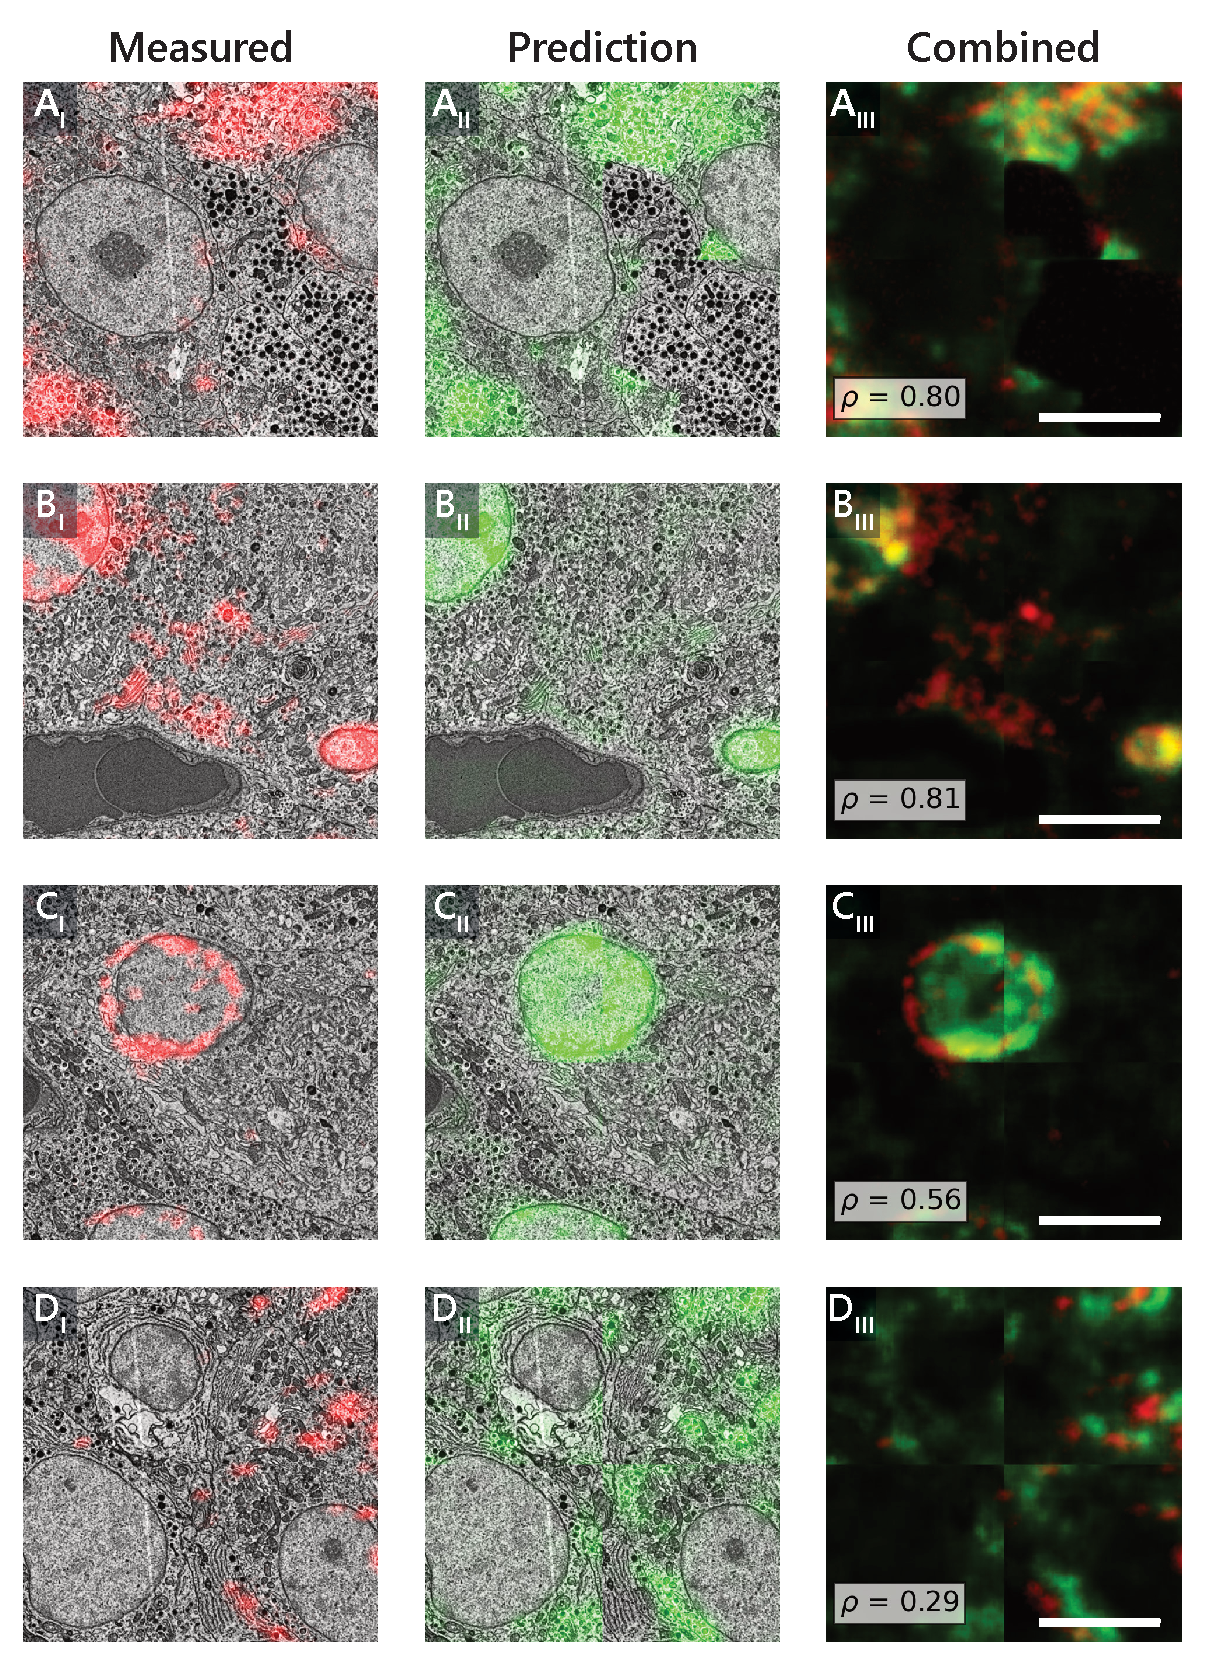
\includegraphics[width=0.95\linewidth]{chapter-4/figures_PDF/fig4-S1_rois.pdf}
    \caption{CLEMnet is able to perform nontrivial structural recognition tasks as well as mitigate issues inherent to fluorescence imaging. (Continued on next page\ldots)}
    \label{fig:4.S1_rois}
\end{figure}
\addtocounter{figure}{-1}
\begin{figure}
    \caption{For each selected ROI (A-D), the measured fluorescence (left, red) and prediction (center, green) are overlaid onto the EM, and combined to show overlap and differences in signal intensity (right).
    (A) The network is able to distinguish between insulin and similar-looking glucagon granules, a difficult task for non-experts.
    (B) An instance of AF594 emission from \SI{405}{\nano\meter} Hoechst excitation demonstrates that the network prediction is less susceptible to bleedthrough. 
    (C) As the network generates predictions directly on structures within the EM, it is able to compensate for errors in the EM-FM registration near the edges of the field of view where the registration may be extrapolated.
    (D) The network is for the same reason also less susceptible to off-axis aberrations such as vignetting, which results in diminished signal at the corners of the fluorescence field of view.
    Note that several predictions are stitched together to compose the predicted image shown, at times giving rise to edge artefacts.
    Scale bars: (A--D) \SI{5}{\micro\meter}.}
\end{figure}

\quad


% References
\printbibliography[title={References}]
